\FloatBarrier
\par En las figuras \ref{fig:ej2-1core} y \ref{fig:ej2-2core} se pueden ver los gr\'aficos de Gantt para el lote de tareas de este ejercicio, para 1 y 2 cores, respectivamente.
\par La latencia para un solo core es de 4 ciclos de CPU para la taskCPU, 109 ciclos para una de las tasksConsola y 190 ciclos para la otra.
Para dos cores es de 4 ciclos para la taskCPU y una de las tasksConsola y de 85 para la otra.
\par Con los resultados de la figura \ref{fig:ej2-1core} se puede ver claramente el problema que puede surgir al utilizar un scheduler First Come First Serve: el usuario en este tipo de casos esperar\'ia poner a correr su algoritmo, y pasar el tiempo hasta que \'este termine de ejecutarse utilizando otras aplicaciones. 
Sin embargo, al correr este lote de tareas en una computadora con un solo core se debe esperar a que termine de correr la primer tarea para poder utilizar otras aplicaciones. 
Si bien con otro tipo de scheduler (por ejemplo Round Robin) el algoritmo tardar\'ia m\'as tiempo, el usuario podr\'ia utilizar otras aplicaciones mientras tanto para hacer pasar el tiempo.
\par Al emplear dos cores para correr el lote de tareas se alivia el problema detallado previamente, ya que al menos se puede ejecutar una de las aplicaciones deseadas mientras corre el algoritmo CPU-intensivo en el otro core, como se ve en la figura \ref{fig:ej2-2core}.
Sin embargo, el problema no se elimina completamente debido a que a\'un se debe esperar a que la primera aplicaci\'on termine de ejecutar para poder correr la segunda.
La \'unica forma de eliminar completamente este problema para un scheduler FCFS es tener a disposici\'on m\'as cores que tareas a ejecutar, pero s\'olo en raras circunstancias es posible satisfacer este requerimiento.
\begin{figure}[h]
\caption{Lote de tareas de Rolando para 1 core}
\label{fig:ej2-1core}
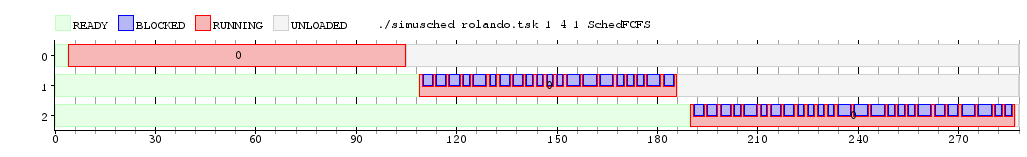
\includegraphics[width=0.9\columnwidth]{imgs/ej2-1core}
\end{figure}
\begin{figure}[h]
\caption{Lote de tareas de Rolando para 2 cores}
\label{fig:ej2-2core}
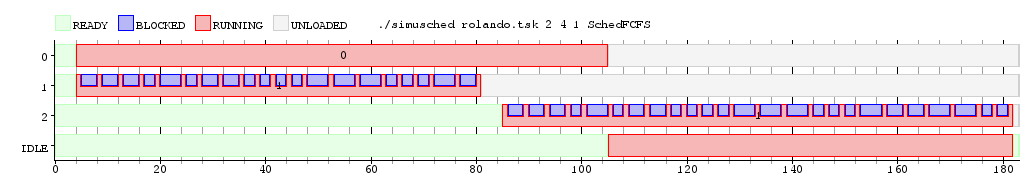
\includegraphics[width=0.9\columnwidth]{imgs/ej2-2core}
\end{figure}
\FloatBarrier
